% ============================================================
%  Team-Finder — Software Engineering Document
%  Compile: pdflatex Team_Finder_Documentation.tex  (run twice)
%  Images required:
%    assets/workflow.png  — export from WORKFLOW_INTERACTIVE.html
%    assets/erd.png       — already present
% ============================================================

\documentclass[12pt,a4paper]{article}

% --- Encoding & Font -------------------------------------------
\usepackage[utf8]{inputenc}
\usepackage[T1]{fontenc}
\usepackage{lmodern}
\usepackage{microtype}

% --- Page Geometry ---------------------------------------------
\usepackage{geometry}
\geometry{a4paper, top=2.5cm, bottom=2.5cm, left=3cm, right=2.5cm}

% --- Graphics & Color ------------------------------------------
\usepackage{graphicx}
\usepackage{xcolor}
\usepackage{tikz}
\usetikzlibrary{calc}

\definecolor{tfpurple}{RGB}{88,28,135}
\definecolor{tfblue}{RGB}{30,58,138}
\definecolor{tflightblue}{RGB}{59,130,246}
\definecolor{tfgray}{RGB}{107,114,128}
\definecolor{tforange}{RGB}{154,52,18}
\definecolor{rowgray}{RGB}{245,245,245}

% --- Hyperlinks ------------------------------------------------
\usepackage[
  colorlinks=true,
  linkcolor=tfblue,
  urlcolor=tflightblue,
  citecolor=tfblue,
  pdftitle={Team-Finder Software Engineering Document},
  pdfauthor={Team-Finder Development Team}
]{hyperref}

% --- Table of Contents Styling ---------------------------------
\usepackage{tocloft}
\renewcommand{\cftsecfont}{\bfseries\color{tfblue}}
\renewcommand{\cftsecpagefont}{\bfseries\color{tfblue}}
\renewcommand{\cftsubsecfont}{\color{tfblue}}
\renewcommand{\cftsubsecpagefont}{\color{tfblue}}
\renewcommand{\cftsubsubsecfont}{\color{tforange}}
\renewcommand{\cftsubsubsecpagefont}{\color{tforange}}
\setlength{\cftsecindent}{0pt}
\setlength{\cftsubsecindent}{1.5em}
\setlength{\cftsubsubsecindent}{3.2em}
\setcounter{tocdepth}{3}

% --- Section Heading Styles ------------------------------------
\usepackage{titlesec}
\titleformat{\section}
  {\large\bfseries\color{tfblue}}
  {\thesection}{1em}{}[\vspace{2pt}\color{tfblue}\titlerule]
\titleformat{\subsection}
  {\normalsize\bfseries\color{tfblue}}
  {\thesubsection}{1em}{}
\titleformat{\subsubsection}
  {\normalsize\bfseries\color{tforange}}
  {\thesubsubsection}{1em}{}

\titlespacing*{\section}{0pt}{16pt}{8pt}
\titlespacing*{\subsection}{0pt}{12pt}{4pt}
\titlespacing*{\subsubsection}{0pt}{10pt}{3pt}

% --- Tables ----------------------------------------------------
\usepackage{booktabs}
\usepackage{longtable}
\usepackage{array}
\usepackage{tabularx}
\usepackage{multirow}
\newcolumntype{L}[1]{>{\raggedright\arraybackslash}p{#1}}
\newcolumntype{C}[1]{>{\centering\arraybackslash}p{#1}}

% --- Math ------------------------------------------------------
\usepackage{amsmath}
\usepackage{amssymb}

% --- Headers & Footers -----------------------------------------
\usepackage{fancyhdr}
\pagestyle{fancy}
\fancyhf{}
\fancyhead[L]{\small\color{tfgray} Team-Finder}
\fancyhead[R]{\small\color{tfgray} Software Engineering Document}
\fancyfoot[C]{\small\thepage}
\renewcommand{\headrulewidth}{0.4pt}
\renewcommand{\footrulewidth}{0pt}

% --- Spacing ---------------------------------------------------
\usepackage{setspace}
\usepackage{parskip}
\setlength{\parskip}{6pt}
\setlength{\parindent}{0pt}

% --- Floats & Captions ----------------------------------------
\usepackage{float}
\usepackage{caption}
\captionsetup{font=small, labelfont=bf, labelsep=period}

% --- Listings (code blocks) ------------------------------------
\usepackage{listings}
\lstset{
  basicstyle=\ttfamily\small,
  backgroundcolor=\color{rowgray},
  frame=single,
  framerule=0.4pt,
  rulecolor=\color{tfgray},
  breaklines=true,
  captionpos=b
}

% --- Misc ------------------------------------------------------
\usepackage{enumitem}
\setlist{noitemsep, topsep=3pt}

% ============================================================
%  DOCUMENT START
% ============================================================
\begin{document}

% ------------------------------------------------------------
%  COVER PAGE
% ------------------------------------------------------------
\begin{titlepage}

  % Full-bleed purple header via TikZ overlay
  \begin{tikzpicture}[remember picture, overlay]
    \fill[tfpurple]
      (current page.north west)
      rectangle
      ($ (current page.north east) + (0,-9cm) $);
    \node[
      anchor=center,
      text=white,
      font=\fontsize{54}{64}\selectfont\bfseries
    ] at ($ (current page.north) + (0,-4.5cm) $) {Team-Finder};
  \end{tikzpicture}

  \vspace{10cm}

  \noindent\textbf{\large University of Jordan}
  \hfill
  \textbf{\large IT Department}

  \vspace{5.5cm}

  \noindent Aws Hanaqtah \hfill 0234960 \\[5pt]
  \noindent Mohammad Rababa'ah \hfill 0244154 \\[5pt]
  \noindent Saif Indrawes \hfill 0239332 \\[5pt]
  \noindent Rafat Malkawi \hfill 0236257 \\[5pt]
  \noindent Nour Al-Bustanjee \hfill 0234089 \\[5pt]
  \noindent Khaled Saadeh \hfill 0233786

\end{titlepage}

% ------------------------------------------------------------
%  TABLE OF CONTENTS
% ------------------------------------------------------------
\newpage
\thispagestyle{plain}
\tableofcontents

% ============================================================
%  SECTION 1 — PROJECT INITIATION
% ============================================================
\newpage
\section{Project Initiation}

\subsection{Project Overview}

Team-Finder is a university student team-matching platform that connects students based on
verified academic profiles, technical skill assessments, and collaboration availability.
The platform is currently deployed for students at the University of Jordan and the
Hashemite University, authenticated through their institutional email domains
(\texttt{ju.edu.jo} and \texttt{hu.edu.jo}). The architecture is designed for institutional
extensibility: adding a new university requires only registering its email domain in the
authentication layer, with no structural changes to the database or application logic.

The system addresses three interconnected needs. First, team formation: students discover
collaborators through a skill-based matching engine that scores student-to-project fit using
cosine similarity on skill vectors, normalized peer ratings, and availability alignment,
producing a ranked compatibility score on a 0--100 scale. Second, learning: students access
a curated catalog of university courses, developer tooling, and personalized career roadmaps
derived from the open-source roadmap.sh project. Third, AI-assisted guidance: a conversational
career assistant backed by Anthropic Claude and the LangGraph agent framework helps students
manage their academic profile, browse projects, plan their semester, and navigate their
learning trajectory.

Version 1 of the platform was published approximately one year prior to this document.
The current version constitutes a major rebuild, introducing approximately 65 percent new
functionality including the AI assistant subsystem, the full learning page, an adaptive
skill assessment mechanism, and a fully redesigned responsive frontend.

The system is built on a three-layer architecture: a Next.js 14 frontend handling
client-side rendering and direct Supabase database reads, a Python FastAPI backend
hosting the LangGraph AI agent, and a Supabase PostgreSQL database with Row-Level
Security enforced on all tables.

The complete user journey from authentication through profile completion to project
discovery, learning, and AI assistance is shown in Figure~\ref{fig:workflow}.

\begin{figure}[H]
  \centering
  \IfFileExists{assets/workflow.png}{%
    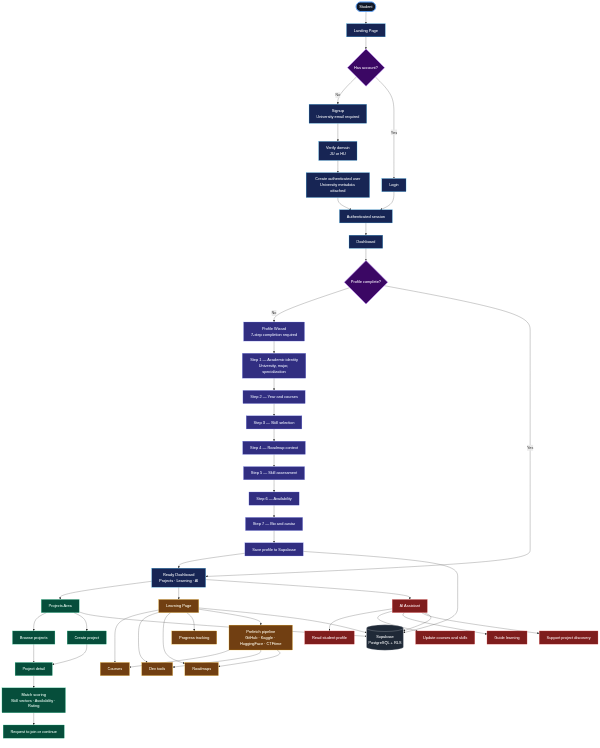
\includegraphics[width=\textwidth]{assets/workflow.png}%
  }{%
    \fbox{\begin{minipage}{0.95\textwidth}
      \centering\vspace{1.5cm}
      {\color{tfgray}\textit{[Workflow Diagram --- export
        docs/WORKFLOW\_INTERACTIVE.html as docs/assets/workflow.png]}}
      \vspace{1.5cm}
    \end{minipage}}%
  }
  \caption{Team-Finder system workflow. Full user journey from authentication through
    profile completion, project discovery, learning, and AI assistance.}
  \label{fig:workflow}
\end{figure}

\subsection{Problem Definition}

\subsubsection{Current Situation and Problem Statement}

University students forming project teams today rely entirely on informal social channels.
At the University of Jordan and the Hashemite University the prevailing methods are
WhatsApp group messages, in-class announcements, and asking acquaintances directly.
These methods are bounded by social network size: a student's access to potential
collaborators is limited to people they already know, not people who are the best
technical fit for the work. No university-provided system exists for structured teammate
discovery, no mechanism exists to express or verify technical skill levels in any
standardised way, and informal channels carry no academic context such as major, year,
course history, or availability when teams are formed.

\subsubsection{Issues}

The core problems driving this project are three. Students have no structured way to find
teammates beyond their immediate social circle. There is no mechanism to verify whether a
student actually possesses a claimed technical skill at any meaningful proficiency level.
All existing informal channels carry no academic context, meaning there is no concept of
major, year, completed courses, or collaboration availability when teams are assembled.

\subsubsection{Objectives for Each Issue}

To resolve the absence of structured teammate discovery, Team-Finder builds a skill-based
matching engine that scores student-to-project fit using cosine similarity on binary skill
vectors, normalized peer ratings, and availability, producing a ranked compatibility score
from 0 to 100. To resolve the absence of skill verification, the platform implements a
multi-level internal assessment mechanism with adaptive difficulty covering Beginner,
Intermediate, and Advanced levels across 38 technical skills in 7 categories. To resolve
the absence of academic context, every matching and discovery decision is anchored on
verified profile data including major, academic year, semester, and completed course history.

\subsubsection{General System Requirements}

The platform must be accessible across iOS mobile devices, desktop browsers, and web
clients with a fully responsive interface. All data operations must be authenticated and
authorised through Supabase Row-Level Security policies. The AI assistant must verify
user identity on every request via a signed JWT before accessing or modifying any data.
The system must support the full profile wizard flow, project browsing and filtering,
learning resource access, and real-time AI conversation within the same authenticated
session, with no functionality gated behind non-free-tier infrastructure.

\subsubsection{Constraints}

The platform operates under three distinct constraint categories.

On the client side, the system must function correctly across iPhone and iOS browsers,
desktop browsers, and web clients. No server-side rendering dependency may break mobile
compatibility, and all interactive components must be touch-accessible.

On the budget side, the project carries zero allocated funding. All development is unpaid
student work. The only external cost incurred is the Claude Code development environment
subscription used during implementation. All production services operate on free-tier
accounts: Supabase free tier (500\,MB database storage, 50\,MB file storage,
2\,GB monthly bandwidth) and the Anthropic Claude API on a monitored paid key.

On the schedule side, the delivery deadline for this version is two weeks from the date
of this document.

\subsection{Feasibility Study}

\subsubsection{Technical Feasibility}

The full technology stack is proven and production-grade. Next.js 14 with the App Router,
FastAPI, Supabase PostgreSQL, and the Anthropic Claude API are all actively maintained
frameworks with large developer communities and well-documented integration patterns. The
LangGraph agent framework is purpose-built for multi-tool conversational agents and has
an established integration path with the Anthropic SDK. All inter-layer integrations
follow established patterns: the Supabase JavaScript client in the frontend, PyJWT-based
JWT verification in the backend, and a direct PostgreSQL connection via psycopg2 for
agent write operations. The platform has already been running in a prior version,
confirming the stack is viable in this deployment context.

\subsubsection{Operational Feasibility}

After delivery, the platform will be operated by the product owner or under the terms of
any acquisition or licensing agreement. The system requires no active human administration
for normal operation. Database maintenance, authentication, and hosting are delegated to
Supabase. AI inference is handled by the Anthropic API. The only ongoing operational
concern is monitoring API token usage and Supabase bandwidth consumption against free-tier
limits as the user base scales.

\subsubsection{Economic Feasibility}

The project carries zero direct financial cost to the development team. All services are
either free-tier or covered by existing subscriptions. The Anthropic API operates on a
pay-per-use model; current usage during development remains within acceptable cost ranges.
The economic model for production deployment is undetermined and market-dependent, with
potential paths including university licensing agreements or a subscription-based access
model.

\subsubsection{Schedule Feasibility}

Version 1 of the platform was published approximately one year prior to this document.
The current version is a major rebuild introducing approximately 65 percent new
functionality. The target delivery date for this version is two weeks from the date of
this document. Given that core infrastructure is already operational and the majority of
features are implemented and tested, this timeline is feasible.

\subsubsection{Legal Feasibility}

The platform stores student names, institutional email addresses, academic records, and
availability data in a Supabase-managed PostgreSQL instance on third-party infrastructure.
Compliance with any specific data protection regulation or university-level data governance
policy is the responsibility of the purchasing or licensing institution. The platform
architecture supports migration to a self-hosted Supabase instance if institutional policy
requires data residency.

\subsection{Recommended Solution and Expected Deliverables}

The recommended solution is the Team-Finder platform in its current state: a fully
operational, responsive web application with university-gated authentication, a seven-step
profile wizard, a client-side skill-based matching engine, a learning page with courses
and roadmaps, and an AI career assistant. The expected deliverables are the working
platform with all implemented features active and all security measures enforced, together
with this software engineering document.

\subsection{Local and Global Impact}

Locally, the platform addresses a gap in Jordan's higher education ecosystem where no
structured tool exists for student team formation. Adoption by Jordanian universities
could improve project output quality, reduce team formation friction, and support a
collaborative engineering culture among students. A commercial path exists through direct
university acquisition or a subscription-based access model; the specifics are
market-dependent.

Globally, the platform architecture is not region-specific. The university domain
verification system accommodates any institution by registering its email domain. The
skill catalog, roadmap integration, and AI assistant are language- and institution-agnostic.
The scope of international expansion is currently undetermined and contingent on market
reception.

\subsection{Naming Conventions and Definitions}

\begin{longtable}{@{} L{3.5cm} L{11cm} @{}}
\toprule
\textbf{Term} & \textbf{Definition} \\
\midrule
\endfirsthead
\toprule
\textbf{Term} & \textbf{Definition} \\
\midrule
\endhead
\bottomrule
\endlastfoot
JU          & University of Jordan (\texttt{ju.edu.jo}) \\[2pt]
HU          & Hashemite University (\texttt{hu.edu.jo}) \\[2pt]
RLS         & Row-Level Security --- PostgreSQL access control enforced at the database layer \\[2pt]
JWT         & JSON Web Token --- signed token used for stateless API authentication \\[2pt]
MCQ         & Multiple Choice Question \\[2pt]
API         & Application Programming Interface \\[2pt]
SRS         & Software Requirements Specification \\[2pt]
WBS         & Work Breakdown Structure \\[2pt]
LLM         & Large Language Model \\[2pt]
AI          & Artificial Intelligence \\[2pt]
UI          & User Interface \\[2pt]
SSR         & Server-Side Rendering \\[2pt]
CSR         & Client-Side Rendering \\[2pt]
V1          & Version 1 --- the original Team-Finder release published approximately one year prior to this document \\[2pt]
Profile gate & The requirement that a student must complete the profile wizard before project discovery and matching are unlocked \\[2pt]
Skill lock  & A rule preventing a student from claiming a skill before reaching the required academic year or completing a prerequisite course \\
\end{longtable}

% ============================================================
%  SECTION 2 — PROJECT MANAGEMENT PLAN
% ============================================================
\newpage
\section{Project Management Plan}

\subsection{Project Organization}

The project is developed by a team of six students from the IT Department at the
University of Jordan. The team operates without a formal hierarchical management
structure. Responsibilities are distributed by technical domain, with each member
accountable for their assigned area. Development communication is conducted through
GitHub commits and pull requests for code changes, WhatsApp for asynchronous team
coordination, and one formal in-person meeting held during the project lifecycle.

\subsection{Roles and Responsibilities}

\begin{longtable}{@{} L{4.5cm} L{10cm} @{}}
\toprule
\textbf{Team Member} & \textbf{Responsibilities} \\
\midrule
\endfirsthead
\toprule
\textbf{Team Member} & \textbf{Responsibilities} \\
\midrule
\endhead
\bottomrule
\endlastfoot
Aws Hanaqtah        & Frontend development, backend development, system architecture, API design, database integration \\[4pt]
Mamoun              & AI agent integration, LangGraph toolchain configuration, Claude API tool design, system prompt engineering \\[4pt]
Amro                & Quality assurance, functional testing, test case design \\[4pt]
Mohammad Rababa'ah  & Quality assurance, functional testing \\[4pt]
Saif Indrawes       & Technical documentation \\[4pt]
Rafat Malkawi       & Technical documentation \\[4pt]
Nour Al-Bustanjee   & Technical documentation \\[4pt]
Khaled Saadeh       & Technical documentation \\
\end{longtable}

\subsection{Software Process Model}

The project follows the Scrum framework operating within an Agile methodology.
Development is organized into iterative sprints with continuous integration of
new features. Requirements are treated as a living backlog, prioritized by
technical dependency and delivery risk. Testing and documentation occur in
parallel with feature development rather than as a sequential phase. This model
was selected because the platform requirements evolved substantially during
development, and the iterative Scrum cycle allowed the team to accommodate new
feature specifications, architectural changes, and UI redesigns without
discarding prior work.

\subsection{Tools and Techniques}

\begin{longtable}{@{} L{3.5cm} L{11cm} @{}}
\toprule
\textbf{Tool} & \textbf{Purpose} \\
\midrule
\endfirsthead
\toprule
\textbf{Tool} & \textbf{Purpose} \\
\midrule
\endhead
\bottomrule
\endlastfoot
GitHub          & Version control, branch management, code review \\[2pt]
VS Code         & Primary development environment \\[2pt]
Next.js 14      & Frontend framework --- App Router, TypeScript, TailwindCSS \\[2pt]
FastAPI         & Backend REST API framework \\[2pt]
LangGraph       & AI agent state machine and tool orchestration \\[2pt]
Supabase        & PostgreSQL database, authentication, Row-Level Security \\[2pt]
Anthropic API   & Claude Sonnet 4 LLM powering the AI career assistant \\[2pt]
psycopg2        & Direct PostgreSQL connection for AI agent write operations \\[2pt]
PyJWT           & JWT verification for Supabase tokens in the FastAPI backend \\[2pt]
WhatsApp        & Asynchronous team communication \\[2pt]
LaTeX           & Technical documentation typesetting \\
\end{longtable}

\subsection{Work Breakdown Structure}

\begin{longtable}{@{} C{1.2cm} L{4cm} L{9.3cm} @{}}
\toprule
\textbf{ID} & \textbf{Work Package} & \textbf{Tasks} \\
\midrule
\endfirsthead
\toprule
\textbf{ID} & \textbf{Work Package} & \textbf{Tasks} \\
\midrule
\endhead
\bottomrule
\endlastfoot
1.0 & Requirements \& Planning     & System requirements analysis, database schema design, API contract definition \\[4pt]
2.0 & Core Infrastructure           & Supabase project setup and migrations, authentication system, Next.js scaffold, FastAPI scaffold \\[4pt]
3.0 & Profile Wizard                & Seven-step wizard UI, localStorage draft persistence, skill lock system, profile completion gate \\[4pt]
4.0 & Skill Assessment              & Internal MCQ engine, adaptive difficulty logic, retake cooldown, confidence rating calculation \\[4pt]
5.0 & Project Discovery \& Matching & Project browsing UI, client-side cosine similarity engine, difficulty filters, project creation flow \\[4pt]
6.0 & Learning Page                 & Course catalog, dev tools hub, roadmap viewer, learning progress tracking, roadmap.sh seed script \\[4pt]
7.0 & AI Assistant                  & LangGraph agent, 14-tool inventory, JWT-authenticated FastAPI endpoint, thread ownership enforcement \\[4pt]
8.0 & Data Pipeline                 & External project prefetcher, roadmap seeder, dev tool seeder \\[4pt]
9.0 & Testing \& QA                 & Functional test cases, cross-platform testing (iOS, desktop, web), security verification \\[4pt]
10.0 & Documentation \& Delivery    & Software engineering document, final deployment validation \\
\end{longtable}

\subsection{Assigning Team Members to Tasks}

\begin{longtable}{@{} L{3.5cm} L{11cm} @{}}
\toprule
\textbf{Team Member} & \textbf{Assigned Work Packages} \\
\midrule
\endfirsthead
\toprule
\textbf{Team Member} & \textbf{Assigned Work Packages} \\
\midrule
\endhead
\bottomrule
\endlastfoot
Aws Hanaqtah        & 1.0, 2.0, 3.0, 4.0, 5.0, 6.0, 8.0 \\[2pt]
Mamoun              & 7.0 \\[2pt]
Amro                & 9.0 \\[2pt]
Mohammad Rababa'ah  & 9.0 \\[2pt]
Saif Indrawes       & 10.0 \\[2pt]
Rafat Malkawi       & 10.0 \\[2pt]
Nour Al-Bustanjee   & 10.0 \\[2pt]
Khaled Saadeh       & 10.0 \\
\end{longtable}

\subsection{Project Schedule}

\begin{longtable}{@{} L{4.5cm} L{10cm} @{}}
\toprule
\textbf{Phase} & \textbf{Timeline} \\
\midrule
\endfirsthead
\toprule
\textbf{Phase} & \textbf{Timeline} \\
\midrule
\endhead
\bottomrule
\endlastfoot
V1 Development          & Completed approximately twelve months prior to this document \\[2pt]
V2 Planning \& Rebuild  & Eight weeks prior to delivery --- architecture redesign, new feature specification \\[2pt]
Feature Implementation  & Weeks 3--10 --- profile wizard, matching engine, learning page, AI assistant, data pipeline \\[2pt]
Testing \& QA           & Weeks 9--12 --- parallel with late feature development \\[2pt]
Documentation           & Final two weeks --- software engineering document, deployment validation \\[2pt]
Final Delivery          & Two weeks from date of this document \\
\end{longtable}

\subsection{Risk Analysis and Plans}

\begin{longtable}{@{} L{4.5cm} L{5.5cm} L{4.5cm} @{}}
\toprule
\textbf{Risk} & \textbf{Description} & \textbf{Mitigation} \\
\midrule
\endfirsthead
\toprule
\textbf{Risk} & \textbf{Description} & \textbf{Mitigation} \\
\midrule
\endhead
\bottomrule
\endlastfoot
Supabase free tier limits &
  500\,MB database and 2\,GB bandwidth cap may be reached under concurrent university-scale load &
  Monitor usage dashboard; migrate to paid tier under licensing or acquisition contract \\[6pt]
Anthropic API cost scaling &
  Per-token billing means AI assistant usage costs grow linearly with active users &
  Implement request rate limiting per user session; cache repeated tool results where safe \\[6pt]
In-memory agent state &
  The LangGraph MemorySaver checkpointer stores conversation state in process memory; a server restart loses all active threads &
  Migrate to a persistent checkpointer (PostgreSQL-backed) before production scaling \\
\end{longtable}

\subsection{Monitoring, Reporting, and Controlling Mechanisms}

Development progress is tracked through GitHub commit history and branch activity,
which provides a continuous audit trail of changes by contributor. Asynchronous
coordination and issue discussion are conducted via the team WhatsApp group. One formal
in-person meeting was held during the project lifecycle to align on architecture decisions
and task distribution. No automated CI/CD pipeline is currently configured; build
verification is performed manually before merging to the main branch.

% ============================================================
%  SECTION 3 — SOFTWARE REQUIREMENTS SPECIFICATIONS
% ============================================================
\newpage
\section{Software Requirements Specifications}

\subsection{System Stakeholders and Requirement Source}

The primary stakeholders are university students at JU and HU who use the platform to
build profiles, discover projects, find teammates, and access learning resources. The
secondary stakeholders are university administrators and academic supervisors who may
evaluate platform adoption or oversee student project formation. Requirements were derived
from direct observation of the current informal team-formation process, analysis of
comparable platforms, and iterative development feedback during V1 operation.

\subsection{User Requirements and Stories}

As a student, I want to register with my university email so that my institutional
affiliation is verified before I can access the platform.

As a student, I want to build a structured academic profile so that other students and
projects can find me based on my actual skills, year, and availability.

As a student, I want to verify my technical skills through a formal assessment so that
my profile reflects real proficiency rather than self-reported claims.

As a student, I want to browse projects filtered by difficulty and technology so that I
can identify opportunities that match my current skill level.

As a student, I want to receive a ranked match score against a project so that I
understand how well my profile fits before applying to join.

As a student, I want to access structured learning resources tied to my major and skills
so that I can develop the competencies needed for the projects I am targeting.

As a student, I want to interact with an AI assistant that knows my academic profile so
that I can get personalised guidance on courses, skills, and career planning.

\subsection{Use Case Model}

The system defines three primary actors: the Unauthenticated Visitor, who can only access
the landing page; the Authenticated Student with an incomplete profile, who is restricted
to the profile wizard; and the Authenticated Student with a complete profile, who has full
access to the dashboard, projects, learning page, and AI assistant. The core use cases
are User Registration (UC-01), Profile Completion (UC-02), and Skill Assessment (UC-03).
Project discovery, learning access, and AI chat are downstream use cases unlocked only
after profile completion.

\subsection{Functional Requirements Specification}

\subsubsection{Authentication and Account Management}

\textit{Status: Implemented.}

The platform restricts registration to email addresses belonging to supported university
domains. At signup, the system validates that the provided email ends in \texttt{ju.edu.jo}
or \texttt{hu.edu.jo} and attaches the corresponding university identifier to the user's
authentication metadata in Supabase. This university field is immutable after creation:
the database UPDATE policy on the \texttt{profiles} table includes a CHECK constraint that
rejects any attempt to change the \texttt{university}, \texttt{email}, or
\texttt{verification\_method} columns, even by the authenticated user themselves.

Session management is handled entirely by Supabase Auth. The frontend middleware refreshes
the Supabase session on every request. The Python backend independently verifies the
Supabase-issued JWT on every API call using the \texttt{SUPABASE\_JWT\_SECRET}, validating
the token's signature, expiry, issuer, and audience before extracting the user identifier.
The user identity used by the AI agent is always taken from the verified JWT, never from
the request body.

\subsubsection{Profile Management}

\textit{Status: Implemented.}

The profile wizard is a seven-step sequential flow that a student must complete before
project discovery and matching are unlocked. Draft state is saved to browser localStorage
after each step using a versioned schema with a seven-day expiry, allowing a student to
resume the wizard across sessions.

Step 1 captures university, major, and specialization. Step 2 captures academic year,
current semester, and completed courses selected from the university's course catalog.
Step 3 presents the skill selector, where skills are gated by a lock system: each of
the 38 catalogued skills has a \texttt{requiredYear} field and a list of course IDs that
unlock it. A student below the required year cannot claim the skill unless they have
completed an unlocking course. Year 1 students receive C\texttt{++} at Beginner level by
default. Step 4 captures roadmap and project context. Step 5 is the skill assessment
(described separately in UC-03). Step 6 captures availability preference from four
options: Full-time, Flexible, Evenings, or Weekends. Step 7 captures bio text and assigns
an avatar colour from the platform palette.

A profile is considered complete when the student has set a major, set their academic year,
added at least three skills, and recorded at least one completed course. Until all four
criteria are satisfied, the project discovery area is locked and the dashboard shows the
completion checklist.

\subsubsection{Skill Search and Matching}

\textit{Status: Implemented.}

Project discovery is available to students with complete profiles. The dashboard presents
two project categories: university projects created by students at the same institution,
and external projects seeded from the data prefetching pipeline. Projects can be filtered
by difficulty level (Beginner, Intermediate, Advanced) and searched by title, description,
or technology stack.

The matching engine runs entirely on the client side in the browser. For a given project
and student, the score is computed as follows. Each skill set is encoded as a binary vector
of length equal to the full skill catalog. Cosine similarity is computed between the project
skill vector and the student skill vector. The final score is a weighted sum:

\begin{equation}
  \text{score} =
    \Bigl(\text{cosine}(\vec{v}_{\text{project}},\, \vec{v}_{\text{student}}) \times 0.60\Bigr)
    + \Bigl(\frac{\text{rating}}{5} \times 0.25\Bigr)
    + \Bigl(\text{avail}_{\text{norm}} \times 0.15\Bigr)
\end{equation}

If the student's normalised rating is below 0.40 (equivalent to a 2-out-of-5 rating), a
penalty multiplier of 0.50 is applied to the total score, halving it. The final result is
rounded to an integer in the range $[0,\, 100]$.

\subsubsection{AI Assistant}

\textit{Status: Implemented.}

The AI career assistant is accessible as a floating chat panel on the dashboard. The
frontend sends the user's message, the conversation history, and a thread identifier to
\texttt{POST /api/chat} on the FastAPI backend. The backend verifies the JWT, extracts
the user's identifier and university from the token claims, and passes this identity as
immutable configuration into the LangGraph agent. The agent is a singleton instance
cached in process memory and powered by Claude Sonnet~4 (\texttt{claude-sonnet-4-20250514}).

The agent has access to 14 tools organised into four groups. The three profile tools are
\texttt{get\_my\_profile}, \texttt{get\_learning\_progress}, and
\texttt{mark\_learning\_item\_complete}. The four read tools are \texttt{search\_courses},
\texttt{search\_skills\_catalog}, \texttt{get\_available\_projects}, and
\texttt{find\_teammates}. The four write tools are \texttt{add\_course\_to\_student},
\texttt{remove\_course\_from\_student}, \texttt{add\_skill\_to\_student}, and
\texttt{remove\_skill\_from\_student}. The three utility tools are \texttt{get\_major\_plan},
\texttt{search\_roadmap}, and \texttt{get\_available\_roadmaps}.

The write surface is strictly bounded to the authenticated student's own records in the
\texttt{user\_courses}, \texttt{user\_skills}, and \texttt{learning\_progress} tables.
The agent cannot modify any other student's data, cannot write to projects or profiles
directly, and cannot execute raw SQL. Thread identifiers are prefixed with the user's UUID
to prevent cross-user thread access.

The \texttt{find\_teammates} tool returns only name, major, year, availability, and
matched skills. Email addresses and contact information are never returned.

\subsubsection{Learning Page}

\textit{Status: Implemented.}

The learning page is organised into four sub-areas. The course catalog presents all
university courses for the student's major and institution, grouped by year and semester,
with completion status derived from the student's \texttt{user\_courses} record. The dev
tools hub provides curated links to GitHub guides, DevDocs, and practical development
tooling seeded into the \texttt{dev\_tools} and \texttt{dev\_tool\_resources} tables. The
roadmap viewer renders personalised career roadmaps sourced from roadmap.sh, with nodes
the student can mark complete. Learning progress is persisted in the
\texttt{learning\_progress} table and is readable by the AI assistant.

Roadmap content is seeded by \texttt{backend/scripts/seed\_roadmaps.py}, which fetches
node layout JSON and markdown content files from the
\texttt{kamranahmedse/developer-roadmap} GitHub repository and inserts them into the
\texttt{roadmaps}, \texttt{roadmap\_nodes}, and \texttt{roadmap\_node\_resources} tables.
Thirty roadmaps are currently seeded, covering role-based paths (Frontend, Backend,
DevOps, Cyber Security, AI Engineer, etc.) and skill-based paths (Docker, Kubernetes,
AWS, Java, C\texttt{++}, Git, etc.).

\subsubsection{Data Security}

\textit{Status: Implemented.}

All 15 tables in the database have Row-Level Security enabled. The security model enforces
three guarantees at the database layer regardless of application-level behaviour.
First, university affiliation is immutable: the \texttt{profiles} UPDATE policy includes a
WITH CHECK clause that rejects any modification to the \texttt{university},
\texttt{email}, or \texttt{verification\_method} columns. Second, users can only read or
write their own private data: all \texttt{user\_*} tables and assessment results enforce
\texttt{auth.uid() = user\_id} on write operations. Third, project ownership is enforced:
only the creator of a project can update or delete it, and only project owners can manage
membership.

The entity-relationship diagram showing all table relationships is provided in
Figure~\ref{fig:erd}. The complete RLS policy inventory follows in
Table~\ref{tab:rls}.

\begin{figure}[H]
  \centering
  \IfFileExists{assets/erd.png}{%
    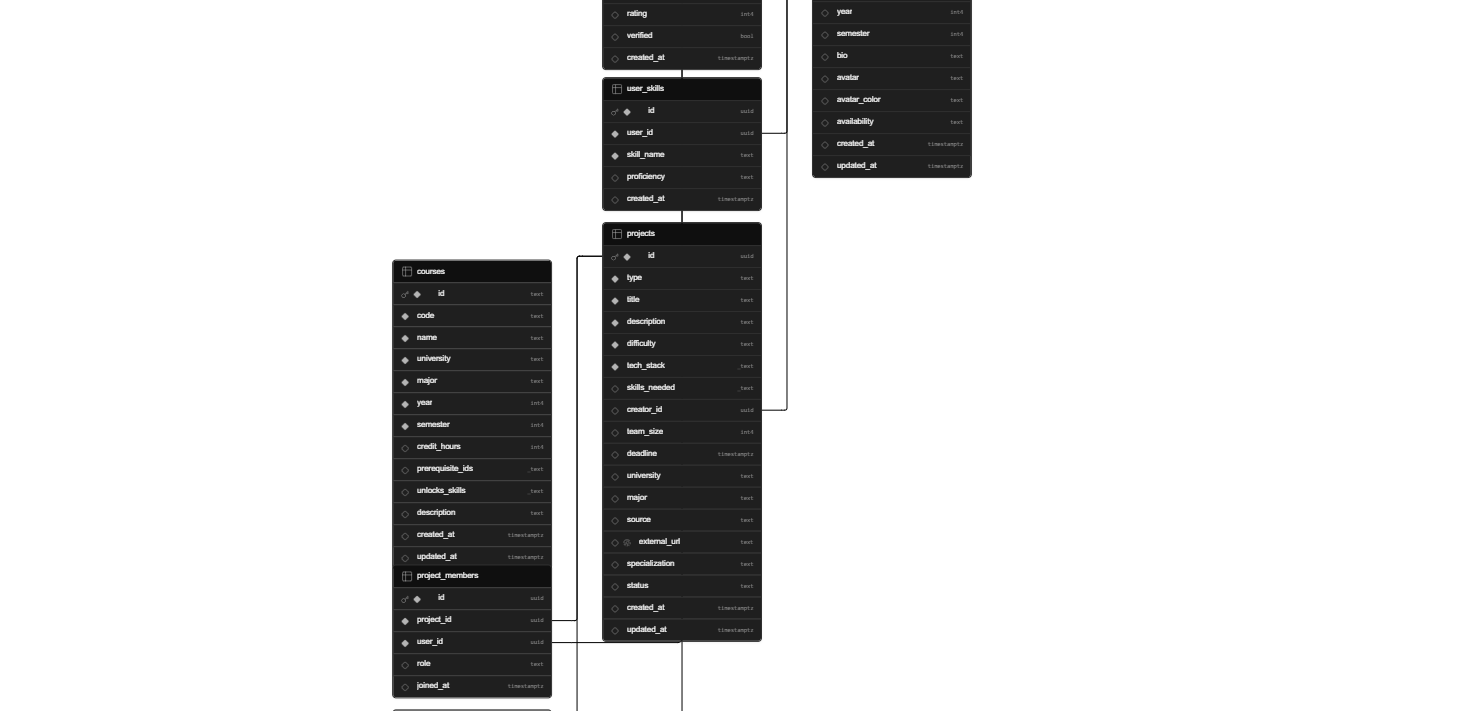
\includegraphics[width=\textwidth]{assets/erd.png}%
  }{%
    \fbox{\begin{minipage}{0.95\textwidth}
      \centering\vspace{1.5cm}
      {\color{tfgray}\textit{[ERD --- file assets/erd.png not found]}}
      \vspace{1.5cm}
    \end{minipage}}%
  }
  \caption{Team-Finder canonical entity-relationship diagram. Tables are grouped by
    domain: user identity, skills, courses, projects, and learning.}
  \label{fig:erd}
\end{figure}

\begin{longtable}{@{} L{3.2cm} L{2.2cm} L{8.8cm} @{}}
\caption{Row-Level Security policy inventory.}
\label{tab:rls} \\
\toprule
\textbf{Table} & \textbf{Operation} & \textbf{Policy} \\
\midrule
\endfirsthead
\toprule
\textbf{Table} & \textbf{Operation} & \textbf{Policy} \\
\midrule
\endhead
\bottomrule
\endlastfoot
profiles            & SELECT  & Public read --- all profiles are visible to authenticated users \\
profiles            & INSERT  & \texttt{auth.uid() = id} --- a user may only create their own profile \\
profiles            & UPDATE  & Own profile only; WITH CHECK rejects changes to \texttt{university}, \texttt{email}, \texttt{verification\_method} \\[4pt]
user\_skills        & SELECT  & Public read \\
user\_skills        & ALL     & \texttt{auth.uid() = user\_id} \\[4pt]
user\_courses       & SELECT  & Public read \\
user\_courses       & ALL     & \texttt{auth.uid() = user\_id} \\[4pt]
courses             & SELECT  & Public read \\
courses             & ALL     & Authenticated users (admin-managed catalog) \\[4pt]
skills              & SELECT  & Public read \\[4pt]
skill\_proficiencies & SELECT & Public read \\
skill\_proficiencies & ALL    & \texttt{auth.uid() = user\_id} \\[4pt]
assessment\_results & SELECT  & \texttt{auth.uid() = user\_id} --- private to owner \\
assessment\_results & INSERT  & \texttt{auth.uid() = user\_id} \\[4pt]
projects            & SELECT  & Public read \\
projects            & INSERT  & \texttt{auth.uid() = creator\_id} AND \texttt{type = 'university'} \\
projects            & UPDATE  & \texttt{auth.uid() = creator\_id} \\
projects            & DELETE  & \texttt{auth.uid() = creator\_id} \\[4pt]
project\_members    & SELECT  & Public read \\
project\_members    & ALL     & Project owner only (subquery on \texttt{project\_members.role = 'owner'}) \\[4pt]
project\_applications & SELECT & Applicant OR project creator \\
project\_applications & INSERT & \texttt{auth.uid() = applicant\_id} \\
project\_applications & UPDATE & Project creator only \\[4pt]
learning\_progress  & SELECT  & \texttt{auth.uid() = user\_id} \\
learning\_progress  & INSERT  & \texttt{auth.uid() = user\_id} \\
learning\_progress  & DELETE  & \texttt{auth.uid() = user\_id} \\[4pt]
roadmaps, roadmap\_nodes, roadmap\_node\_resources, roadmap\_edges & SELECT & Public read (admin-seeded, no user writes permitted) \\[4pt]
dev\_tools, dev\_tool\_resources & SELECT & Public read (admin-seeded, no user writes permitted) \\
\end{longtable}

\subsubsection{Peer-to-Peer Learning}

\textit{Status: Planned.}

The peer-to-peer learning area will provide a structured environment for students to ask
technical questions, receive answers from peers, and contribute course materials. The
design combines a StackOverflow-style question-and-answer system with a tutoring layer
where experienced students can offer guidance in specific subjects. Students will be able
to upload past exam papers and course PDFs, which the AI assistant will use as source
material for generating contextually relevant quiz questions. This feature is not yet
implemented.

\subsubsection{Team Chat}

\textit{Status: Planned.}

The team chat system will provide project-scoped communication channels allowing team
members to coordinate work, assign tasks within the platform, and track project activity
without relying on external messaging tools. A general friend-to-friend chat layer will
also be available alongside project channels. This feature is not yet implemented.

\subsubsection{AI Quiz Generation}

\textit{Status: Planned.}

The AI assistant will generate skill-specific quiz questions on demand, drawing from a
pre-generated question bank stored in the database. Questions will be tagged by skill,
difficulty level, and type (multiple choice or code-reading). The generation process will
run at server startup via a seed script using Claude to produce a minimum of 80 questions
per skill per difficulty level. An adaptive difficulty engine will adjust question
selection within a session based on the student's running answer accuracy, and a
per-question timer will be enforced to reduce the viability of external lookups during
assessment. This feature is not yet implemented.

\subsubsection{Dev Setup Guides}

\textit{Status: Planned.}

The dev tools hub will be extended with structured environment setup guides covering tool
installation (Visual Studio Code, Git, Python, pip, Node.js) and configuration for each
major technology stack used in university projects. Guides will link to official
download pages and verified documentation sources. This feature is partially implemented
through the existing \texttt{dev\_tools} table and \texttt{DevToolsHub} component, with
the full setup guide content pending.

\subsection{Use Case Descriptions}

\subsubsection*{UC-01: User Registration}

\begin{longtable}{@{} L{3.5cm} L{11cm} @{}}
\toprule
\textbf{Field} & \textbf{Detail} \\
\midrule
\endfirsthead
\toprule
\textbf{Field} & \textbf{Detail} \\
\midrule
\endhead
\bottomrule
\endlastfoot
Use Case ID     & UC-01 \\[2pt]
Name            & User Registration \\[2pt]
Actor           & Unauthenticated student \\[2pt]
Precondition    & Student possesses a valid JU or HU institutional email address \\[2pt]
Main Flow       &
  1. Student navigates to the signup page. \newline
  2. Student enters email and password. \newline
  3. System validates the email domain against the supported domain list (\texttt{ju.edu.jo}, \texttt{hu.edu.jo}). \newline
  4. System creates an authenticated Supabase user with the university identifier attached to auth metadata. \newline
  5. System redirects the student to the dashboard. \\[2pt]
Alternative Flow &
  Domain not supported: registration is rejected with an error message stating that only institutional emails are accepted. \\[2pt]
Postcondition   & Authenticated session established with university metadata attached; student is redirected to the profile wizard. \\
\end{longtable}

\vspace{1em}
\subsubsection*{UC-02: Profile Completion}

\begin{longtable}{@{} L{3.5cm} L{11cm} @{}}
\toprule
\textbf{Field} & \textbf{Detail} \\
\midrule
\endfirsthead
\toprule
\textbf{Field} & \textbf{Detail} \\
\midrule
\endhead
\bottomrule
\endlastfoot
Use Case ID     & UC-02 \\[2pt]
Name            & Profile Completion \\[2pt]
Actor           & Authenticated student with incomplete profile \\[2pt]
Precondition    & Authenticated session exists; profile does not yet satisfy the completion criteria \\[2pt]
Main Flow       &
  1. System detects incomplete profile and presents the seven-step wizard. \newline
  2. Student completes each step; draft state is saved to localStorage after each step. \newline
  3. On final submission, the system writes the profile, courses, skills, and assessment results to Supabase. \newline
  4. System evaluates the four completion criteria (major set, year set, minimum three skills, minimum one course). \newline
  5. Profile is marked complete; project discovery and matching are unlocked. \\[2pt]
Alternative Flow &
  Student abandons the wizard mid-flow: the draft persists in localStorage for seven days, allowing the student to resume. If the draft expires, the student restarts from Step 1. \\[2pt]
Postcondition   & Profile is complete; full dashboard access including projects, learning, and AI assistant is granted. \\
\end{longtable}

\vspace{1em}
\subsubsection*{UC-03: Skill Assessment}

\begin{longtable}{@{} L{3.5cm} L{11cm} @{}}
\toprule
\textbf{Field} & \textbf{Detail} \\
\midrule
\endfirsthead
\toprule
\textbf{Field} & \textbf{Detail} \\
\midrule
\endhead
\bottomrule
\endlastfoot
Use Case ID     & UC-03 \\[2pt]
Name            & Skill Assessment \\[2pt]
Actor           & Authenticated student during profile wizard Step 5 \\[2pt]
Precondition    & Student has selected at least one skill in Step 3; skill is unlocked for their year level \\[2pt]
Main Flow       &
  1. Student selects a skill and a difficulty level (Beginner, Intermediate, or Advanced). \newline
  2. System presents a timed multiple-choice exam. The total exam time limit is four minutes. \newline
  3. Student submits answers. \newline
  4. System scores the exam (0--100), calculates a confidence star rating (1--5), and records the result in \texttt{assessment\_results}. \newline
  5. A passing score (50 or above) marks the skill as verified and updates the student's \texttt{skill\_proficiencies} record with the earned rating. \\[2pt]
Alternative Flow &
  Score below 50: skill is recorded as attempted but unverified. A retake is not permitted for seven days from the attempt timestamp (\texttt{retake\_allowed\_at}). \\[2pt]
Postcondition   & Assessment result is stored; skill confidence rating is updated in the student's profile; result is visible to the AI assistant via \texttt{get\_my\_profile}. \\
\end{longtable}

\subsection{Non-Functional Requirements}

\subsubsection{Performance Requirements}

Standard page loads must complete within three seconds on a typical university broadband
connection. API responses from the FastAPI backend for non-AI operations must complete
within two seconds. AI assistant responses, which involve LLM inference and one or more
database tool calls, must complete within ten seconds under normal load. The client-side
matching algorithm, operating entirely in the browser, must produce scores for up to
50 projects in under 200 milliseconds.

\subsubsection{Reliability and Availability}

Platform availability is dependent on the Supabase service level agreement, which
guarantees 99.9 percent uptime for paid-tier projects. The current deployment on the
Supabase free tier does not carry a formal SLA. The FastAPI backend is a single process
with no redundancy; a restart is required to recover from an unhandled exception.
Conversation state held in the LangGraph MemorySaver is lost on process restart.

\subsubsection{Security Requirements}

All write operations to the database are protected by Row-Level Security policies that
enforce user identity at the database layer, independent of application logic. The
university field on a user profile is immutable at the database level. All API endpoints
on the FastAPI backend require a valid Supabase JWT; the user identifier is always
extracted from the token, never from the request body. The AI agent's write surface is
restricted to \texttt{user\_courses}, \texttt{user\_skills}, and \texttt{learning\_progress}
for the authenticated user only. The \texttt{find\_teammates} tool never returns email
addresses or contact information.

\subsubsection{Usability Requirements}

The platform must be fully usable on iOS mobile browsers, desktop browsers, and web
clients without requiring a native application install. The profile wizard must be
completable by a new student in under 15 minutes assuming no technical difficulties.
All interactive controls must meet minimum touch target sizes for mobile accessibility.
Error states in the profile wizard must present specific, actionable feedback
identifying which field or step requires correction.

\subsubsection{Scalability Requirements}

The current Supabase free-tier instance supports approximately 500 concurrent database
connections and 2\,GB of monthly egress bandwidth. This is sufficient for a pilot deployment
within a single university faculty. Scaling beyond this threshold requires migration to a
paid Supabase instance, which removes the connection and bandwidth caps. The application
architecture introduces no additional scalability bottlenecks: the Next.js frontend is
stateless and can be deployed behind a CDN, and the FastAPI backend is horizontally
scalable once the in-memory agent state is migrated to a persistent checkpointer.

\subsection{Data Requirements}

The platform data model consists of 15 tables organised into five domains.

The identity domain contains \texttt{profiles}, which stores one record per authenticated
user with fields for name, email, university, major, specialization, academic year,
semester, bio, avatar, availability, and timestamps. The university and email fields are
immutable after creation.

The skills domain contains \texttt{skills} (the master catalog, 38 entries),
\texttt{user\_skills} (skills claimed by each student), \texttt{skill\_proficiencies}
(per-student skill level and 0--100 rating), and \texttt{assessment\_results} (exam scores
with original and adjusted difficulty, retake timestamps, and score).

The courses domain contains \texttt{courses} (the master catalog for all 12 supported
majors across JU and HU, with \texttt{unlocks\_skills} arrays linking course completion to
skill eligibility) and \texttt{user\_courses} (courses completed or in progress per student).

The projects domain contains \texttt{projects} (both university-created and externally
seeded, with type, difficulty, tech stack, skills needed, team size, and status),
\texttt{project\_members} (team membership with role), and \texttt{project\_applications}
(join requests with pending/accepted/rejected status).

The learning domain contains \texttt{learning\_progress} (roadmap node and course
completion events per student), \texttt{roadmaps}, \texttt{roadmap\_nodes},
\texttt{roadmap\_node\_resources}, \texttt{roadmap\_edges}, \texttt{dev\_tools}, and
\texttt{dev\_tool\_resources}.

All tables have Row-Level Security enabled. All primary keys are UUID or text identifiers.
Timestamps use \texttt{TIMESTAMPTZ} throughout to avoid timezone ambiguity.

\end{document}
